\subsection{Memory \& Attention}
\label{sub:memoryandattention}
    \textbf{Long-term dependencies: LSTM with peepholes} and \textbf{GRUs}:  
    
    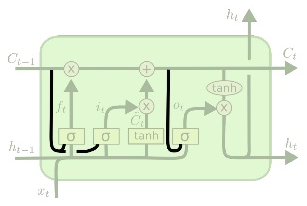
\includegraphics[width=4cm]{images/lstm-peepholes.png}
    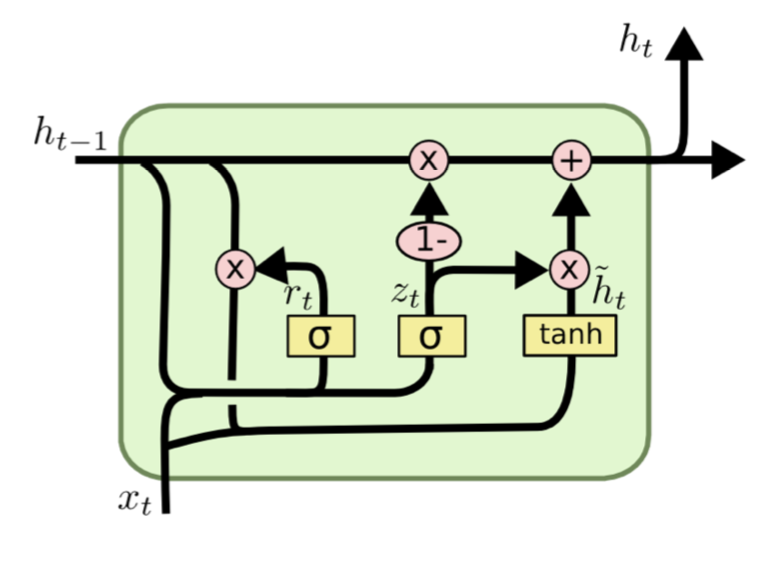
\includegraphics[width=4cm]{images/gru.png}

    
    \tab $i_t=\sigma(W^{(i)}x_t+U^{(i)}h_{t-1})$ input gate\\
\textbf{With peepholes:} $i_t=\sigma(W_i\cdot [C_{t-1},h_{t-1}, x_t]+b_i)$\\
    \tab $o_t=\sigma(W^{(o)}x_t+U^{(o)}h_{t-1})$ output gate \\
\textbf{With peepholes:} $o_t=\sigma(W_o\cdot [C_{t-1},h_{t-1}, x_t]+b_o)$\\
    \tab $f_t=\sigma(W^{(f)}x_t+U^{(f)}h_{t-1})$ forget gate\\
\textbf{With peepholes:} $f_t=\sigma(W_f\cdot [C_{t-1},h_{t-1}, x_t]+b_t)$\\
    \tab $\Tilde{c}_t=\tanh(W^{(c)}x_t+U^{(c)}h_{t-1})$ preparing input to add to memory\\
    \tab $c_t=f_t\odot c_{t-1}+i_t\odot \Tilde{c}_t$ updating memory (combine stored and new)\\
    \tab $h_t=o_t\odot\tanh(c_t)$ output
    
    Where $\odot$ is point-wise multiplication between vectors.
    
    \textbf{Gated memory units:}:

    
    $z_t=\sigma(W_z \cdot [h_{t-1},x_t])$
    $\quad r_t=\sigma(W_r \cdot [h_{t-1},x_t])$\\
    $\Tilde{h}_t=tanh(W \cdot [r_t * h_{t-1},x_t])$
    $\quad h_t=(1-z_t)*h_{t-1}+z_t*\Tilde{h}_t$

    
    \subsubsection{Recursive Networks}
    \label{ssub:recursivenetworks}
    Recurrent = linear chain structure, depth eff. $\vO(n)$, $\vh^t=F(\vh^{t-1},\vx^t)$\\
    Recursive = tree structure, $\vO(\log n)$, $\vh^n=F(\vh^\text{n.left},\vh^\text{n.right})$.\\
    Learn composition $F:\R^d\times\R^d\xrightarrow{}\R^d$, then applied at each inner node of the tree.
